\begin{chapabstract}
\small{
This chapter introduces the concept of anomaly detection for time series analysis, discussing the major existing contributions to the field. This chapter is organized as follows. \autoref{s:anomaly-detection} introduces the definition and properties of time series data and the concept of anomaly. It discusses the several types of techniques existing in the scientific literature, classifying them using a taxonomy. 
\autoref{s:ad-with-dl} focuses on anomaly detection techniques based on deep learning. The method developed in this work belongs to this category.
\autoref{ss:ad-astrophysics} lists several contributions made in the astrophysics field, proving that these techniques are becoming increasingly popular for analyzing astrophysical data.
}\\
\begin{center}
\noindent\makebox[0.8\linewidth]{\rule{0.66\paperwidth}{0.4pt}}
\end{center}
\vspace{1cm}
\end{chapabstract}

\section{Anomaly Detection for time series analysis}
\label{s:anomaly-detection}
Anomaly detection involves the identification of patterns or events in data that are unusual or unexpected compared to a baseline or normal behavior \cite{chandola_2019}. Various factors, such as errors in data collection, rare events, or the influence of external factors, can cause these anomalies. This chapter will discuss anomaly detection in the context of time series data. A time series is generally considered a collection of observations indexed in time order, defined by the following properties:
\begin{itemize}
    \item Temporality (or temporal correlation): if successive data point in the series depends on its past values.
    \item Dimensionality: the number of individual data attributes captured in each observation. In the case of univariate time series, each observation is defined by one data attribute. In contrast, multiple attributes define the observations that compose a multivariate time series. In the latter case, both the temporal dependence and the correlations between data attributes should be considered. Below are the mathematical definitions of a univariate and multivariate time series, assuming that the observations composing a time series have the same temporal granularity.
    \begin{definition} \label{def:univariate-timeseries}
    [Univariate time series] A \textit{univariate time series} $\textbf{X}=\{\textbf{x}_t\}_{t\in T}$ is an ordered set of real-valued observations, where each observation is recorded at a specific time $t \in T \subseteq \mathbb{Z}^+$. 
    \end{definition}
    \begin{definition} \label{def:multivariate-timeseries}
    [Multivariate time series] A \textit{multivariate time series} $\textbf{X}=\{\textbf{x}_t\}_{t\in T}$ is an ordered set of real-valued observations, where each observation is recorded at a specific time $t \in T \subseteq \mathbb{Z}^+$ and consists of k real-valued observations, $\textbf{x}_t = (x_{1t}, .., x_{kt})$. 
    \end{definition}    
    \begin{definition}
    [Subsequence] $\textbf{S}=\{\textbf{x}_p,\textbf{x}_{p+1},..,\textbf{x}_{p+n-1}\}$ is a \textit{subsequence} of length $n \leq |T|$ of a multivariate time series \textbf{X}, for $p,t \in T$ and $p \leq |T| - n + 1$.
    \end{definition}    
    \item Stationarity: a time series is said to be stationary if its statistical properties do not change over time. 
    \begin{definition}
    [Strongly stationary] For any $\tau \in \mathbb{N}$, a continuous stochastic process $\textbf{x}=\{x^t\}_{t \in T \subset \mathbb{Z}^+}$ is strongly stationary if following condition is satisfied:
    $$\bm{F_x}(x^{1+\tau},...,x^{t+\tau})=\bm{F_x}(x^1,...,x^t)$$ 
    where $\bm{F_x}$ denotes the joint distribution function \cite{choi2021deep}.
    \end{definition}    
    Many real-world environments experience changes in their underlying statistical data distribution over time, a phenomenon commonly referred to as concept drift \cite{Widmer_1994}. This can be a significant issue as it can negatively impact the performance of models trained on historical data \cite{Pan_2010}. For example, the \textit{seasonality} is a periodic fluctuation over a limited time scale (e.g., power consumption is high during the day and low during the night, and online sales increase rapidly over the Black Friday weekend and then decrease again). In addition, \textit{change points} are time instants after which the underlying statistical distribution of a stream changes, for example, when operations are stopped and restarted with a different setting. As we will see in the following sections, the scientific literature contains anomaly detection techniques designed to work exclusively with stationary or non-stationary time series, as well as techniques developed for the stationary case and then adapted for the non-stationary setting.
    \item Noise: since it is a common issue in real-world systems, \cite{Tang_2018} adds this property to time series data. The noise is defined as any unwanted signal changes during capture, storage, transmission, processing, or conversion. While noise can often be caused by minor fluctuations in sensor sensitivity and have little impact on the overall data structure, it can make it difficult to distinguish between noise and actual anomalies in a noisy system. This can greatly impact the performance of detection models \cite{Tuzlukov_2002}.
\end{itemize}
     
Before introducing the taxonomy of the anomaly detection techniques for time series data, the definition of anomaly (or outlier) must be given. A widely used definition has been provided by Hawkins \cite{hawkins1980identification}:
\begin{quote}
"An observation which deviates so much from other observations as to arouse suspicions that it was generated by a different mechanism"
\end{quote}
Outliers in time series can have different meanings depending on the context \cite{blazquez2020review}. According to Aggarwal \cite{aggarwal_2016}, they can be seen as noise, erroneous, or unwanted data that are not of interest to the analyst. In these cases, it is best to delete or correct them to improve the data quality. However, in recent years, researchers have increasingly focused on detecting and analyzing unusual but interesting (for a specific domain) phenomena, such as the case of fraud detection. These outliers are often referred to as anomalies. This chapter will refer to this meaning and from now on, the term anomaly will be used. 

The scientific literature proposes numerous anomaly detection techniques applied to time series analysis \cite{chandola_2019}, \cite{blazquez2020review}, \cite{choi2021deep}, \cite{Garg_2021}. In \cite{blazquez2020review} review paper, the anomaly detection techniques are grouped along three axes. The first axis refers to the capability of analyzing univariate or multivariate time series. The second axis refers to the type of anomaly to be detected. Anomalies in time series data can take several forms. A point anomaly is an unusual data point in a specific time instant compared to other values in the series (global) or neighboring points (local). These anomalies can occur in one variable (\textit{O1, O2} in \autoref{fig:point-anomaly}, left panel) or multiple variables (\textit{O1, O2, O3} in \autoref{fig:point-anomaly}, right panel). Another type of anomaly is called subsequence, which refers to consecutive points in time that exhibit unusual behavior together, even if each point is not necessarily an anomaly. These can also be global or local and affect one variable (\textit{O1, O2} in \autoref{fig:subsequence-anomaly}, left panel and \textit{O3} in \autoref{fig:subsequence-anomaly}, right panel) or multiple variables (\textit{O1} in \autoref{fig:subsequence-anomaly}, right panel). Finally, the entire time series can be considered anomalous when multiple variables are involved (\textit{Variable 4} in \autoref{fig:timseries-anomaly}). Although these definitions of anomalies are general and usable in different real-life scenarios, the classification of what is considered abnormal varies based on one's perspective of what is considered normal. Hence they may be further subdivided into more specific groups \cite{choi2021deep}, \cite{Tang_2018}. 

\begin{figure}[t]
\centering
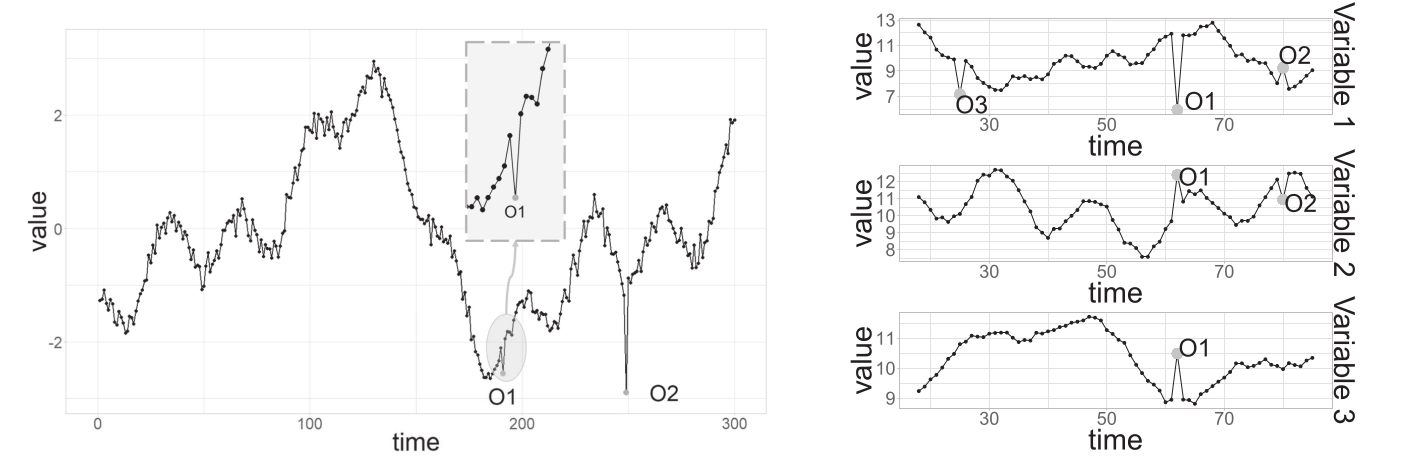
\includegraphics[width=1\linewidth]{figures/introduction-2/point-anomaly.png}
\caption{Point anomalies in time series data. Left panel: univariate time series. Right panel: multivariate time series. Credits to \cite{blazquez2020review}.}
\label{fig:point-anomaly}
\end{figure}
\begin{figure}[t]
\centering
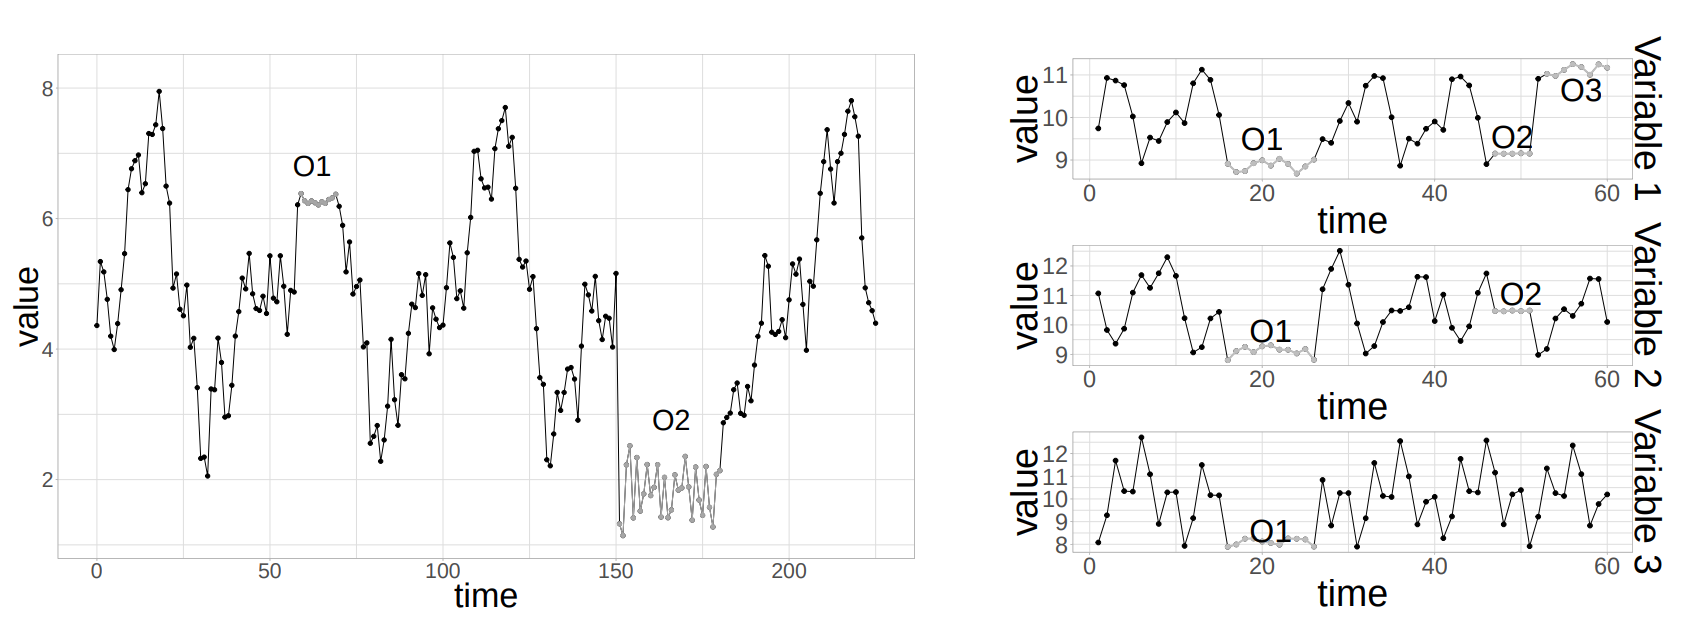
\includegraphics[width=1\linewidth]{figures/introduction-2/subsequence-anomaly.png}
\caption{Subsequence anomalies in time series data. Left panel: univariate time series. Right panel: multivariate time series. Credits to \cite{blazquez2020review}.}
\label{fig:subsequence-anomaly}
\end{figure}
\begin{figure}[t]
\centering
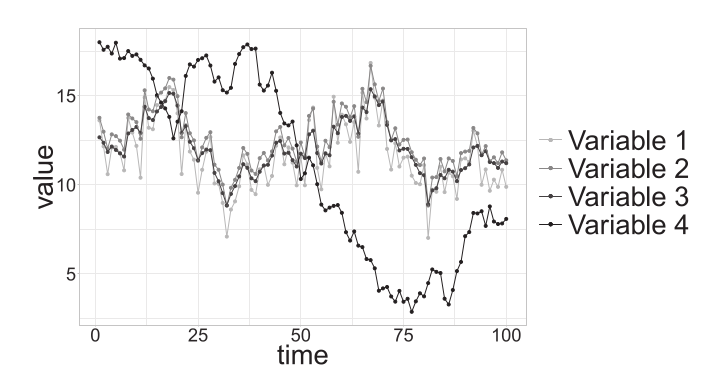
\includegraphics[width=0.6\linewidth]{figures/introduction-2/timseries-anomaly.png}
\caption{Anomalous time series (\textit{Variable 4}) in a multivariate time series. Credits to \cite{blazquez2020review}.}
\label{fig:timseries-anomaly}
\end{figure}

The third dimension of the taxonomy examines the type of detection method used. A univariate detection method only examines one variable over time, while a multivariate method can analyze multiple variables simultaneously. It's worth noting that even though the input data may be a multivariate time series, a univariate detection method can still be employed by analyzing each variable individually, disregarding any potential dependencies between them. However, a multivariate technique cannot be utilized with univariate time series data. Therefore, this dimension only applies to multivariate time series data.

The three dimensions described above are the top nodes of the proposed taxonomy. The authors of \cite{blazquez2020review} further develop the proposed taxonomy tree. In contrast, in \cite{choi2021deep}, the anomaly detection techniques are divided into two main groups: \textit{traditional approaches} and \textit{deep learning based}. The following sections will continue to describe the taxonomy proposed in \cite{blazquez2020review} and then focus on deep learning-based methods mentioned in \cite{choi2021deep}.

\subsection{Anomaly detection techniques for point anomalies in the univariate domain}
\label{ss:point-anomalies-univariate}
The set of anomaly detection techniques that can detect point anomalies is further divided by \cite{blazquez2020review}, taking into account the following aspects:
\begin{itemize}
    \item The technique exploits the \textbf{temporality} of the data: some techniques take into account the temporal ordering of observations, and others completely disregard this information. The latter will produce the same results even when the observations are shuffled.
    \item The technique can be applied in a \textbf{streaming} context: some techniques can identify outliers in real-time, as soon as new data points arrive, without needing to wait for further data. Among these methods, some maintain a constant model throughout the stream. In contrast, others adapt and update their detection models with new information, either by completely retraining the model or through incremental learning. Techniques that cannot make instant decisions on new data points are considered unsuitable for streaming time series analysis.
    \item The \textbf{nature} of the technique: \textit{model-based} techniques rely on fitting a model; \textit{density-based} techniques use the concept of neighborhood; \textit{histogramming} techniques compute a histogram representation of the data. 
\end{itemize}
The next sections will describe further the last point of the previous listing.

\subsubsection{Model-based techniques}
\label{ss:model-based}
The model-based techniques are the most commonly used approach in literature and rely on fitting a model to estimate the expected value of a data point \cite{blazquez2020review}. The data point is considered an anomaly if: 
\begin{definition}\label{def:model-based}
    $|x_t - \hat{x}_t| > \tau $, where $x_t$ is the observed data point and $\hat{x}_t$ is its expected value and $\tau$ is a threshold.
\end{definition}
The expected value, $\hat{x}_t$, represents the typical or normal value of a data point in the time series, and the threshold $\tau$ represents the level of deviation from this normal value considered abnormal or significant. As we will see later in this chapter, \cite{choi2021deep} generalizes this concept with the definition of the \textit{anomaly score}, a numerical value that indicates the likelihood of a data sample being anomalous that replaces the term $|x_t - \hat{x}_t|$ in \autoref{def:model-based}. Despite calculating the expected value $\hat{x}_t$ or the anomaly score and threshold $\tau$ differently, these techniques involve explicitly or implicitly fitting a model. Model-based techniques are divided into \textbf{estimation} (shown in \autoref{fig:model-based}, left panel) and \textbf{prediction} techniques (shown in \autoref{fig:model-based}, right panel). Estimation techniques use $\{x_{t-k_1},...,x_t,...,x_{t+k_2}\}$ to compute $\hat{x}_t$, while in prediction techniques, $\hat{x}_t$ is computed using only previous observations. The main practical difference between the two is that prediction techniques can be applied in the streaming scenario as they can immediately identify whether a new data point is an outlier as soon as it arrives. In contrast, estimation techniques can only do so if only the current point $x_t$ is used to compute the expected value along with some preceding points. 
\begin{figure}[t]
\centering
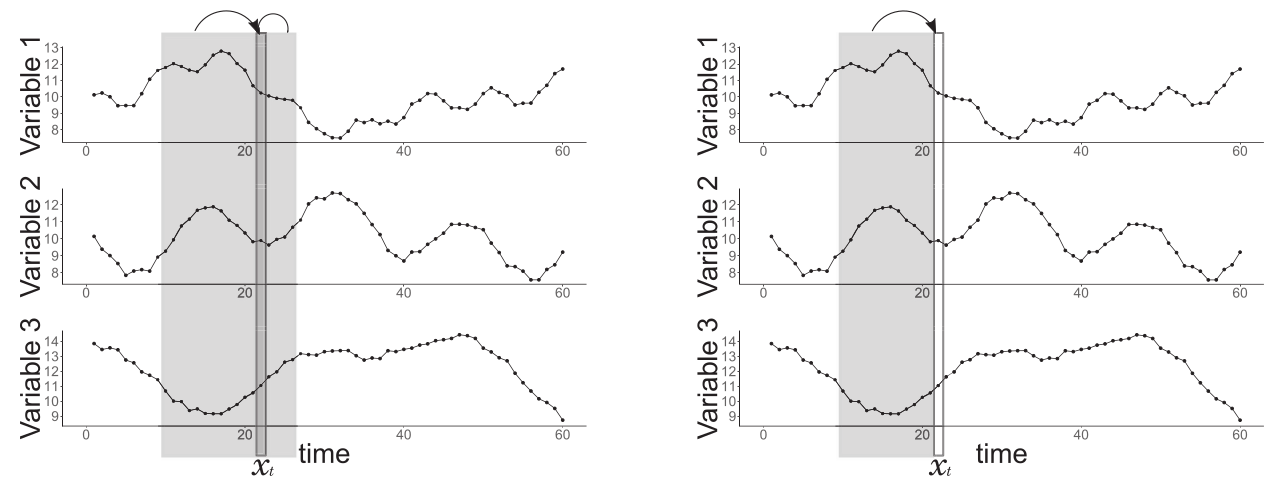
\includegraphics[width=1\linewidth]{figures/introduction-2/model-based.png}
\caption{Example of estimation (left panel) and prediction (right panel) models-based approach for a multivariate time series. Consider only one variable for the univariate scenario. Credits to \cite{blazquez2020review}.}
\label{fig:model-based}
\end{figure}


\subsubsection{Density-based techniques}
The basic idea behind this method is that normal data points will be closely packed together, forming dense clusters. Anomalous data points, on the other hand, will be located in areas of the data where there are few other data points, resulting in a lower density of data in that region. The \textit{density-based} approach relies on computing the density of data points in different regions of the data and identifying any regions with a lower density than the surrounding areas, flagging them as potential anomalies. This approach can be applied to data of any dimensionality and does not rely on prior knowledge of the normal behavior of the data \cite{blazquez2020review}.


\subsubsection{Histogramming techniques}
The method in question is centered around identifying points in a time series that, when removed, result in a histogram representation with less error than the original, even when the number of buckets is decreased to allow for the storage of these points separately (\autoref{fig:histogramming}). This approach aims to detect the points in the time series that deviate from the expected behavior, and removing them allows for a more accurate representation of the data \cite{blazquez2020review}.
\begin{figure}[t]
\centering
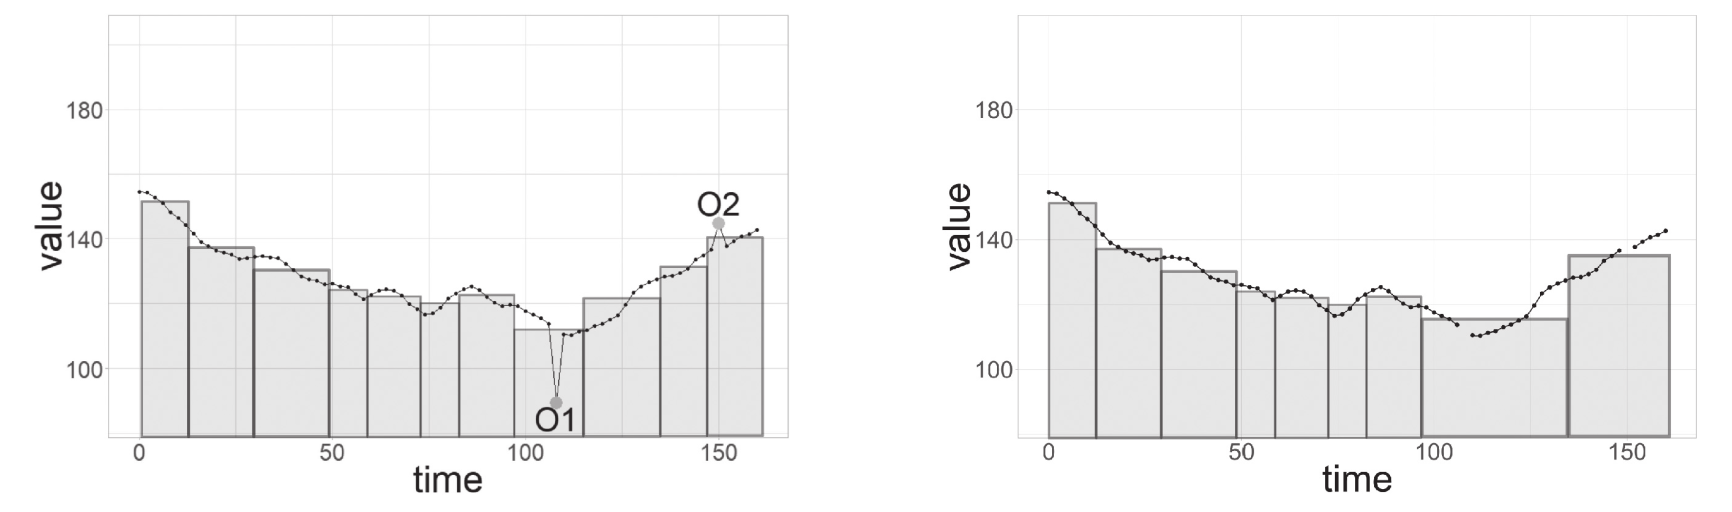
\includegraphics[width=1\linewidth]{figures/introduction-2/histogramming.png}
\caption{Example of the histogramming technique for univariate time series. The points $\{O1, O2\}$ are anomalous. Credits to \cite{blazquez2020review}.}
\label{fig:histogramming}
\end{figure}

\subsubsection{Parametric vs non-parametric techniques}
In \cite{blazquez2020review}, the authors further develop the taxonomy tree taking into account the parametric and non-parametric nature of the techniques. Parametric techniques assume that the underlying distribution of the data belongs to a specific family of distributions and estimate a fixed number of parameters from the data. On the other hand, non-parametric methods do not make any assumptions about the underlying distribution and instead determine the model or family of distributions from the data with a flexible number of parameters. Additionally, there are semi-parametric methods that combine elements of both parametric and non-parametric approaches. In general, the term \textit{anomaly} describes the data points that deviate from the expected behavior. The techniques discussed consider the temporal aspect of the data and can be applied in a streaming context. Additionally, some iterative methods are used to identify and improve the quality of the time series data. Most of the model-based techniques are either parametric or semi-parametric. Semi-parametric techniques typically assume a distribution over the residuals when determining a threshold value, even if the residuals are obtained through a non-parametric approach.

\subsection{Anomaly detection techniques for point anomalies in the multivariate domain}
Multiple variables may be correlated when the input data is composed of multivariate time series. Unlike the case of univariate time series, the detection method used for identifying point outliers in multivariate time series should handle not only a single variable but also multiple variables at once. 
Furthermore, an outlier in a multivariate time series can simultaneously impact one or multiple variables. The set of anomaly detection techniques that can detect point anomalies in the multivariate domain is further divided into two groups by \cite{blazquez2020review}, taking into account the type of analysis: a univariate analysis for each variable to detect univariate point outliers, without considering dependencies that may exist between the variables, or a multivariate analysis, to exploit the correlation dependencies between the variables. Regarding the first case, the techniques described in \autoref{ss:point-anomalies-univariate} can be applied. To overcome the loss of information that occurs when the correlation dependencies between the variables are not considered, dimensionality reduction steps, such as PCA, can be used to find a new set of uncorrelated variables where univariate techniques can be applied. Model-based techniques (prediction and estimation models) and histogramming techniques can be extended to carry out the multivariate analysis. Another model-based technique not cited by \cite{blazquez2020review} but used in the literature (see \autoref{ss:ad-astrophysics}) is called \textit{iForest}, from \cite{Liu_2008}, which is fundamentally different from existing approaches as it explicitly isolates anomalies instead of constructing a profile of normal instances. iForest uses sub-sampling and has a linear time complexity with low constant and memory requirements. It works well, especially in large data sets and high-dimensional problems with many irrelevant attributes. In addition, dissimilarity-based techniques are introduced by \cite{blazquez2020review}.

\subsubsection{Dissimilarity techniques}
\label{ss:dissimilarity-univariate}
These methods involve calculating the difference between multiple points or their representations without needing a model to be fitted. For a set threshold value, if the dissimilarity between a point and its expected value exceeds that threshold, the point is considered an outlier. 
\begin{definition}\label{def:model-based}
    $s(x_t, \hat{x}_t) > \tau $, where $x_t$ is the k-dimensional data point and $\hat{x}_t$ is its expected value and $s$ measures the dissimilarity between two multivariate points.
\end{definition}
These techniques typically do not use raw data but instead employ different representation methods, such as graphs or vectors, and the definition of the dissimilarity function $s$ changes accordingly.



\subsection{Anomaly detection techniques for subsequence anomalies in the univariate domain}
\label{ss:ad-subsequence-univariate}
Subsequence anomalies are the second type of anomaly defined by \cite{chandola_2019}. The objective is to spot a sequence of consecutive points that deviate from normal behavior. In this case, we need to take into account additional aspects. 
\begin{itemize}
    \item First and foremost, unlike point anomalies, subsequences consist of multiple points, introducing a new analysis constraint, i.e., the capability to simultaneously analyze subsequences of varying lengths or rely on fixed-length subsequences. In the latter case, a sliding window over the time series can be used to obtain them. It's also worth noting that the number of subsequences the method will consider and analyze is dependent on the chosen length (i.e. the shorter the length, the higher the number of subsequences). 
    \item Another aspect that subsequence anomaly detection methods must consider is the representation of the data. Since comparing subsequences is more challenging and costly than comparing individual points, many techniques use a representation of the subsequences instead of the raw values, such as the \textit{discretization} method, as shown in \cite{Chandola_2012}.
    \item In addition, the subsequence anomalies can be periodic, making their detection more challenging. Periodic subsequence anomalies are unusual sequences that repeat over time.
    \item Furthermore, instead of point anomaly detection, where some methods do not consider temporal dependencies, subsequences inherently consider temporality.
    \item Finally, when analyzing subsequence anomalies in a streaming context, several approaches can be considered: a single data point arrives, and a classification must be given for a subsequence containing this new point; a subsequence arrives, and it needs to be classified; a batch of data arrives, and subsequence anomalies need to be found within it.
\end{itemize}
In this scenario, the anomaly detection techniques belong to the following groups: 
\textit{discord detection} techniques compare each subsequence to all others using the Euclidean distance and require the user to specify the length of the subsequence. These methods are limited because they cannot specify whether the identified subsequences are anomalies. 
The \textit{dissimilarity-based} techniques in the multivariate scenario use a reference of normality to decide whether or not a subsequence is an anomaly based on their direct comparison. This can be defined as:
\begin{definition}\label{def:dissimilarity-based-multivariate}
    $s(S, \hat{S}) > \tau $, where S is the subsequence being analyzed or its representation, $\hat{S}$ is the expected value of $S$ obtained based on the reference of normality, and $s$ measures the dissimilarity between two subsequences.
\end{definition}
\autoref{fig:dissimilarity} shows some examples of different references of normality ($\hat{S}$ in \autoref{def:dissimilarity-based-multivariate}). The subsequence under analysis ($S$ in \autoref{def:dissimilarity-based-multivariate}) and the references are then clustered, and the centroids or center of the cluster to which the $S$ belongs are computed to identify anomalies (as shown in \autoref{fig:clustering}). The dissimilarity-based techniques in the multivariate scenario differ from those introduced in \autoref{ss:dissimilarity-univariate} because of the representations used to describe subsequences (graphs and vectors against clustered representations).
\begin{figure}[t]
\centering
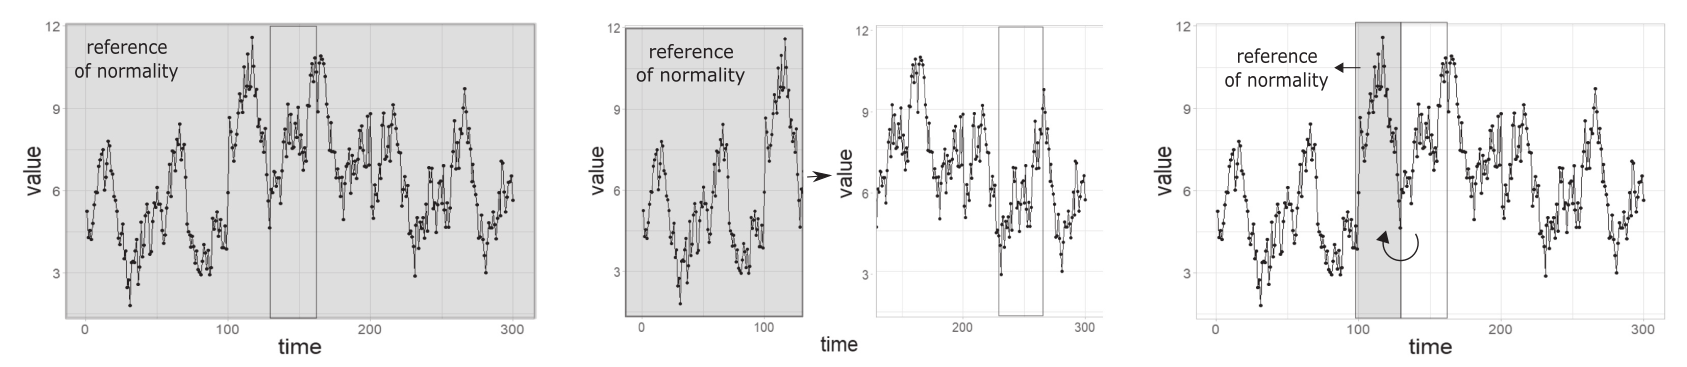
\includegraphics[width=1\linewidth]{figures/introduction-2/dissimilarity.png}
\caption{Example of different references of normality used by dissimilarity-based approaches. The panel on the left shows the same time series. The panel in the middle shows an external time series. The panel on the right shows a previous subsequence. Credits to \cite{blazquez2020review}.}
\label{fig:dissimilarity}
\end{figure}
\begin{figure}[t]
\centering
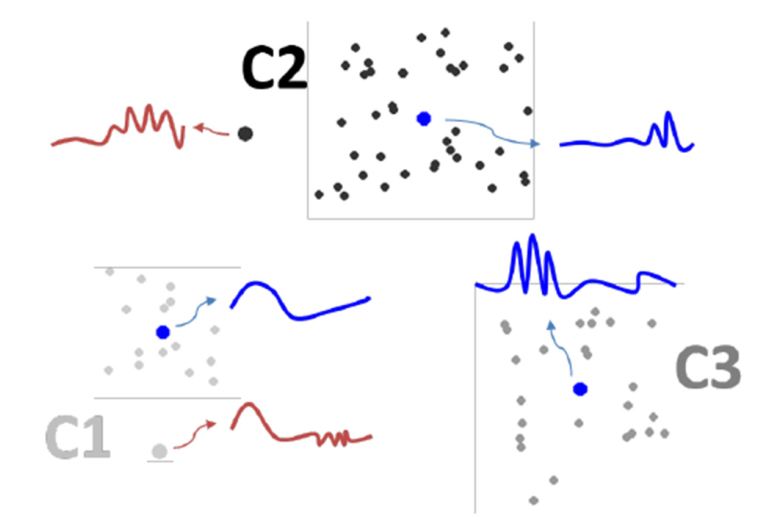
\includegraphics[width=0.5\linewidth]{figures/introduction-2/clustering.png}
\caption{Clustering of the subsequences in a univariate time series. Cluster centroids are highlighted, and C1
and C2 clusters contain subsequence outliers. Credits to \cite{blazquez2020review}.}
\label{fig:clustering}
\end{figure}
The \textit{prediction model-based} techniques in the multivariate scenario build a regression model using past data to predict up to n points into the future. Then, anomalies are detected by calculating the distance from the predicted subsequences to the actual ones. If the distance exceeds a threshold $\tau$ the subsequence is classified as an anomaly. The 
 \textit{frequency-based} techniques compare subsequences to a reference to normality, as done by  \autoref{fig:dissimilarity}. A subsequence $S$ is an
outlier if its frequency is lower than the expected one:
\begin{definition}\label{def:frequency-based}
    $|f(S) - \hat{f}(S)| > \tau $, where $f(S)$ is the frequency of occurrence of $S$, $\hat{f}(S)$ its expected frequency, and $\tau$ a predefined threshold.
\end{definition}
Finally, the last group of multivariate subsequence anomaly detection techniques is based on \textit{information theory}, similar to the frequency-based methods. The main idea is to find patterns in data that happen less often but still happen regularly concerning a reference to normality. Patterns that happen less often are more surprising and carry more information. This can be achieved by looking at how often the symbols in a pattern appeared in the series and how often the pattern appeared overall. 

\subsection{Anomaly detection techniques for subsequence anomalies in the multivariate domain}
\label{ss:ad-subsequence-multivariate}
The techniques mentioned by \cite{blazquez2020review} in this scenario share similar concepts with the technique to detect subsequence anomalies in the univariate domain, as they are simply an advanced version of simpler techniques that have already been discussed earlier. In particular, \textit{model-based} techniques, both prediction and estimation models, performs the best in this scenario, especially if based on deep learning. The following section will focus on this group of techniques.


\section{Anomaly detection with deep learning}
\label{s:ad-with-dl}
To understand why deep learning in unsupervised settings has a critical role in the anomaly detection context, we have two consider two main challenges, described in \cite{choi2021deep}. The first is the rarity of the anomalies. This scarcity makes it time-consuming and resource-intensive to gather enough data for supervised datasets. Additionally, when labeled data is obtained, the imbalance between normal and abnormal data can negatively impact the training of models. In addition, for most real-life use cases, it is not guaranteed to be able to generate a supervised dataset fully representative of the anomalous class. Another challenge regards the complexity of the data. Univariate time-series analysis is still relevant in applications that require minimal computation, such as edge computing. However, as automation and control systems become more complex, it becomes impractical to monitor individual univariate data streams separately. With many dimensions, traditional approaches often experience a decline in performance due to the \textit{curse of dimensionality}. Furthermore, correlations between variables that cannot be inferred through univariate time-series analysis can also indicate anomalies. 



\subsection{Deep learning architectures for anomaly detection in multivariate time series}
The past behavior of a sequence holds valuable information that can indicate potential changes in the future, and deep learning architecture can natively model the temporal context of the data. A popular method is using Recurrent Neural Networks (RNN) and other variants, such as Long Short-Term Memory (LSTM) \cite{Hochreiter_1997} and Gated Recurrent Unit (GRU \cite{Chung_2014}. Those architectures address the vanishing or exploding gradient problem, which occurs when the gradient becomes too small or too large as the network becomes deeper. Through several \textit{gates}, they can learn long-term dependencies by deciding which previous states to keep or discard at each time step. Another approach is the dilated RNN \cite{Chang_2017}, which extracts multi-scale features and models long-term dependencies by using a skip connection between hidden states. While Recurrent Neural Networks (RNNs) are commonly used for analyzing time series data, some studies have found that Convolutional Neural Networks (CNNs) can perform better in certain scenarios that involve short-term data \cite{choi2021deep}. CNNs utilize multiple layers of convolutions, which allow them to learn increasingly complex features as they progress through the layers. 
Additionally, pooling layers introduce non-linearity to the CNNs, allowing them to capture complex patterns \cite{Albawi_2017}. However, a drawback of using CNNs is that it can be challenging to understand patterns that occur over a prolonged period. To address this issue, Temporal Convolutional Networks (TCN) have been proposed by \cite{Lea_2016}. TCN has three distinct characteristics; it uses causal convolutions, meaning that future information is not considered when analyzing past data. It can handle input sequences of any length, similar to RNNs. Furthermore, it can look far into the past using deep networks and dilated convolutions to make predictions. A hybrid architecture, called ConvLSTM, has been introduced by \cite{Shi_2015} to address the spatiotemporal sequence-forecasting problem, i.e., when there's the need to consider the spatial information and temporal dependencies simultaneously.
The spatial information is introduced when a multivariate time series is represented as a 2D covariance matrix. Those matrices are stacked when the time series is monitored with a sliding window, as explained in \cite{choi2021deep}. Recent architectures based on the attention layers \cite{Vaswani_2017}, such as Transformers and bidirectional encoder representations from transformer (BERT) \cite{Devlin_2018}, have been widely used in the field of natural language processing and have recently been applied to the time-series anomaly detection domain due to their ability to handle long-range dependencies effectively. Hierarchical Temporal Memory (HTM) \cite{Hawkins_2016} is a relatively new approach to deep learning architecture and is still being actively researched. HTM has a biologically-inspired design, as it is based on the structure and function of the neocortex, which is the part of the brain responsible for sensory perception, cognition, and decision-making. HTM comprises a hierarchy of layers containing a set of cells organized into columns. The cells in each column are connected to one another and to cells in adjacent columns. The input and the previous states of the connected cells activate the columns. This allows the algorithm to learn and recognize spatial and temporal patterns, making it useful for various applications, including anomaly detection. In addition, one of the key advantages of HTM is its ability to learn and adapt to changing data patterns, making it useful for real-time applications. 

\subsubsection{Anomaly criteria}
\label{ss:anomaly-criteria}
\begin{figure}[t]
\centering
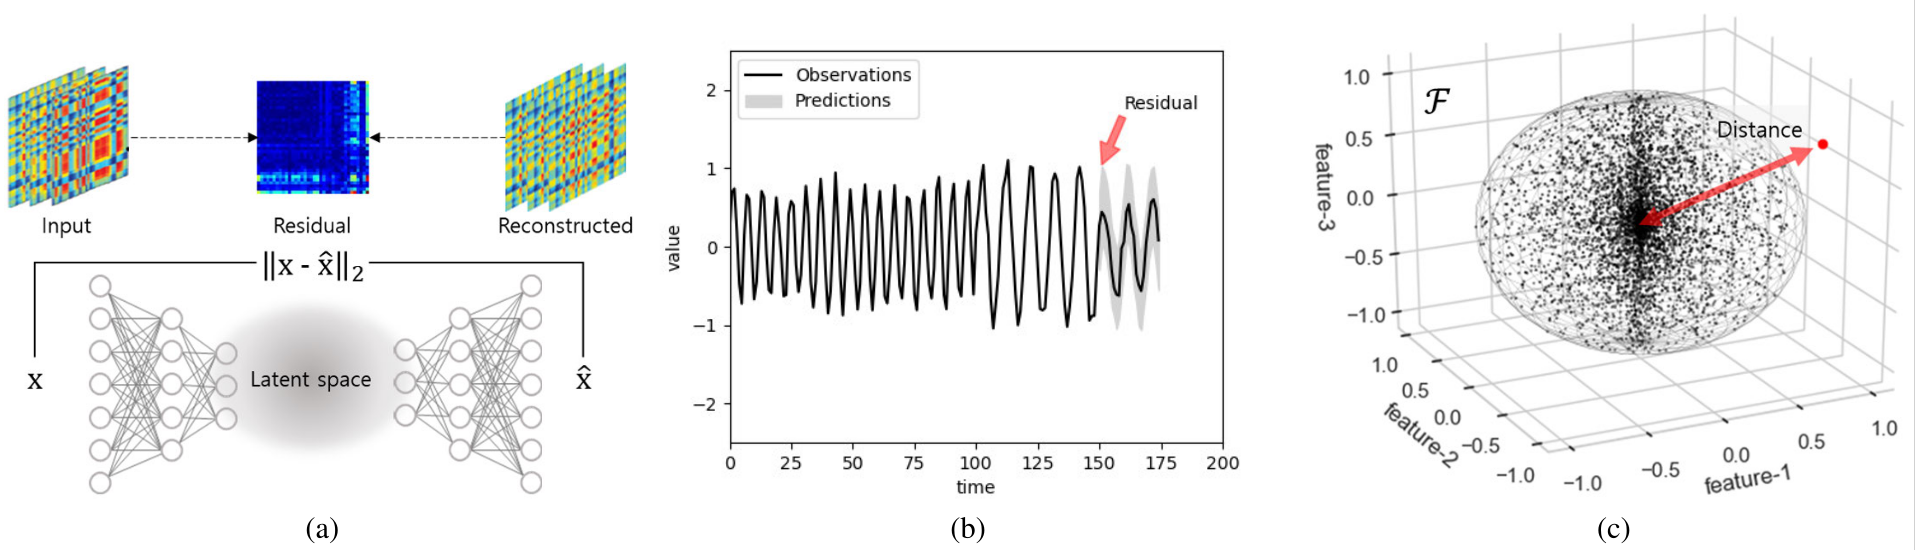
\includegraphics[width=1\linewidth]{figures/introduction-2/anomaly_criteria.png}
\caption{Examples of the anomaly criteria: (a) a reconstruction error; (b) a prediction error; and (c) a dissimilarity. Credits to \cite{choi2021deep}.}
\label{fig:anomaly-criteria}
\end{figure}
The anomaly detection techniques based on deep learning are subdivided into three main categories by \cite{choi2021deep}, concerning the criteria they use to define anomalies. Those techniques all belong to the \autoref{ss:model-based} category introduced in \cite{blazquez2020review}. As outlined in \autoref{ss:model-based}, a model-based technique relies on fitting a model. In this case, a loss function must be defined and minimized since \textit{backpropagation} is used as the learning algorithm. This objective function differs concerning the architecture used. Once the model is trained and the data representation is learned, it is applied to production data to perform inference. The model's output is used to compute an \textit{anomaly score}, i.e., a numerical value that indicates the likelihood of a data sample being anomalous. If the indicator it's greater than a threshold $\tau$, the sample is classified as anomalous. The strategies to compute the anomaly score can be divided into three types: the first is called \textit{recostruction error} and it's a generalization of the estimation-based method described in \autoref{ss:model-based}. This anomaly score is commonly used by AE, VAE, GAN and Transformers. They reconstruct or generate data analogous to the input data and compute the residual between the input and generated data, as shown in \autoref{fig:anomaly-criteria}, panel (a). Prediction techniques compute $\hat{x_t}$ using only previous observations. Obtaining anomaly scores involves assigning a binary label according to the chance of the data point being deemed normal, as outlined in [116], [119]. The discrepancy between the predicted label and actual label demonstrates the prediction error. This method can not always be applied since labels are insufficient in many real-world scenarios. Another method to obtain anomaly scores from prediction models is very similar to \autoref{def:model-based}: the model forecasts the predicted value for future time steps and the anomaly score is computed as the difference between the expected value and the actual data. The latter strategy is shown in \autoref{fig:anomaly-criteria}, panel (b). Finally, the third category contains \textit{dissimilarity-based} methods that extract features from the input data, create clusters, and assess the distance between from the cluster of previous data. This dissimilarity-based method evaluates the similarity through different measures, including the Euclidean distance, Minkowski distance, cosine similarity, and Mahalanobis distance. \cite{choi2021deep} contains several references to techniques that implement the anomaly criteria described above. 

\section{Anomaly detection in astrophysics}
\label{ss:ad-astrophysics}
As automation and technological advancements spread across industries, many systems produce vast amounts of high-dimensional data. As shown by \cite{chandola_2019}, \cite{blazquez2020review}, \cite{choi2021deep}, and \cite{Garg_2021} review papers, anomaly detection techniques are being used in a wide range of contexts, such as identifying fraud in financial transactions, detecting defects in manufacturing processes, identifying cyber attacks in network security, and detecting diseases in medical imaging. These techniques are particularly useful in high-dimensional datasets where manual inspection is infeasible. and when labeled data is unavailable. However, most implementations are highly specific to the individual use case and thus require domain knowledge for appropriate deployment \cite{choi2021deep}. 

The astrophysics domain has the same characteristics: a massive amount of high-dimensional data is being produced, and generating fully-representative supervised datasets is not always feasible due to limited computational resources but also the difficulties in considering all possible sources of systematics, including glitches \cite{Sadeh_2020}, and all possible anomalies, that may be unknown.

Several anomaly detection techniques are used in different astrophysics domains, from traditional methods such as PCA or Isolation Forest to deep learning-based methods. In \cite{Pruzhinskaya_2019}, the photometric data of the Open Supernova Catalog (OSC) is analyzed with dimensionality reduction, and anomalies are detected with the isolation forest algorithm. The latter technique is also the backbone of \textit{Astronomaly} \cite{Webb_2020}, \cite{Lochner_2021}, a general anomaly detection framework with a novel active learning approach designed to provide personalized recommendations for astronomical data, including images, light curves, and spectra. An anomaly detection algorithm based on an unsupervised Random Forest is proposed by \cite{Baron_2017}, which is tested on more than two million galaxy spectra from the Sloan Digital Sky Survey. Furthermore, techniques based on clustering are proposed in the literature \cite{Sadr_2019}, \cite{Giles_2019}. In \cite{Doorenbos_2021}, the performance of six unsupervised outlier detection methods, including the Local Outlier Factor, Isolation Forest, k-means clustering and a convolutional autoencoder, are being compared for the analysis of images from the Sloan Digital Sky Survey. Deep learning-based techniques are also being used: \cite{Ichinohe_2019} proposes an anomaly detection technique based on a variational auto-encoder for high-resolution X-ray spectroscopy, \cite{Margalef_2020} explores the use of deep generative networks for detecting outliers in astronomical imaging data sets, \cite{Zhang_2018} and \cite{Sadeh_2020} use Long Short-term Memory (LSTM). In particular, \cite{Sadeh_2020} proposes a new data-driven discovery framework developed to detect and characterize explosive astrophysical transients using multiple messengers such as neutrinos, optical supernovae, and gamma-rays. Finally, \cite{Marianer_2021} uses semi-supervised outlier detection algorithms to search for unmodelled gravitational wave (GW) signals.